\documentclass[a4paper,12pt]{article}

\title{Chapter 4. Interacting Fields and Feynman Diagrams\\
4-5. Cross Sections and the S-Matrix}
\date{各種SNS\\
    X (旧 Twitter): \href{https://x.com/miya_max_study}{@miya\_max\_study}\\
    Instagram : \href{https://www.instagram.com/daily_life_of_miya/}{@daily\_life\_of\_miya}\\
    YouTube : \href{https://www.youtube.com/@miya-max-active}{@miya-max-active}
    }
\author{Max Miyazaki}

\usepackage{amsmath}
\usepackage{amssymb}
\usepackage{ascmac}
\usepackage{amsthm}
\usepackage{amsfonts}
\usepackage{enumitem}
\usepackage{color}
\usepackage[dvipdfmx]{graphicx}
\usepackage{float}
\usepackage{bm}
\usepackage{here}

\usepackage{abstract}
\usepackage{tikz}
\usetikzlibrary{shapes.geometric, arrows.meta, positioning}
\usepackage{indentfirst}
\usepackage[utf8]{inputenc}
\usepackage{fix-cm}
\usepackage{wrapfig}
\pagenumbering{arabic}
\usepackage{url}
\usepackage{xcolor}
\usepackage[most]{tcolorbox}
\usepackage{framed}
\usepackage[dvipdfmx]{hyperref}
\hypersetup{
 setpagesize=false,
 bookmarksnumbered=true,
 colorlinks=true,
 linkcolor=blue
}

% Define braket-like commands
\newcommand{\bra}[1]{\left\langle #1\right|}
\newcommand{\ket}[1]{\left|#1\right\rangle}
\newcommand{\braket}[2]{\left\langle #1\middle|#2\right\rangle}
\newcommand{\brakets}[3]{\left\langle #1\middle| #2 \middle|#3 \right\rangle}

\renewcommand{\arraystretch}{2.1}


\setlength{\textwidth}{16cm}
\setlength{\textheight}{25cm}
\setlength{\oddsidemargin}{0cm}
\setlength{\evensidemargin}{0cm}
\setlength{\topmargin}{-2cm}

\begin{document}
\maketitle

\vspace{1cm}
\begin{abstract}
    このノートはPeskin\&Schroederの``An Introduction to Quantum Field Theory''の第4章の5節をまとめたものである. 要点や個人的な追記, 計算ノート的なまとめを行っているが, それらはすべて原書の内容を出発点としている. 参考程度に使っていただきたいが, このノートは私の勉強ノートであり, そのままの内容をそのまま鵜呑みにすると間違った理解を招く可能性があることをご了承ください. ぜひ原著を手に取り, その内容をご自身で確認していただくことを推奨します. てへぺろ v$({\hat{\cdot}_\partial \hat{\cdot}})$v
\end{abstract}
    
    

\newpage
\color{blue}
\section*{概要}

\begin{itemize}
  \item \textbf{目標}
  \begin{itemize}
    \item 相互作用場の摂動論を, 時空的過程 (因果律) として視覚化できる形式で発展させる.
    \item まず二点相関関数(グリーン関数)の計算から始める.
  \end{itemize}

  \item \textbf{二点相関関数の定義}
  \begin{itemize}
    \item $\phi^4$ 理論において基底状態 $\lvert \Omega \rangle$ の二点相関関数を考える:
    \begin{equation*}
      \langle \Omega | T\{\phi(x)\phi(y)\} | \Omega \rangle .
    \end{equation*}
    \item 自由理論ではこれはファインマン伝播子に一致する.
  \end{itemize}

  \item \textbf{相互作用の導入}
  \begin{itemize}
    \item Hamiltonian を $H = H_0 + H_{\text{int}}$ に分け, 相互作用を摂動として扱う.
    \item 相互作用表示を用いて, 自由場 $\phi_I$ を基礎に展開する.
  \end{itemize}

  \item \textbf{時間発展演算子 $U(t,t_0)$}
  \begin{itemize}
    \item ハイゼンベルク場 $\phi$ は
    \begin{equation*}
      \phi(t,\mathbf{x}) = U^\dagger(t,t_0)\phi_I(t,\mathbf{x})U(t,t_0)
    \end{equation*}
    で表される.
    \item $U(t,t_0)$ は Dyson 展開で表現される:
    \begin{equation*}
      U(t,t_0) = T \exp\left[ -i\int_{t_0}^t dt' \, H_I(t') \right].
    \end{equation*}
  \end{itemize}

  \item \textbf{基底状態 $\lvert \Omega \rangle$ の構成}
  \begin{itemize}
    \item 相互作用を含む基底状態は, 自由理論の真空 $\lvert 0 \rangle$ を時間発展させることで得られる.
    \item 大きな $T$ の極限をとることで, 基底状態 $n=0$ の項のみが残る.
  \end{itemize}

  \item \textbf{二点相関関数の最終式}
  \begin{itemize}
    \item 相関関数は真空期待値で表される:
    \begin{equation*}
      \langle \Omega | T\{\phi(x)\phi(y)\} | \Omega \rangle
      = \lim_{T \to \infty (1-i\epsilon)}
      \frac{\langle 0 | T \{ \phi_I(x)\phi_I(y)\exp[-i\int_{-T}^T dt\, H_I(t)] \} | 0 \rangle}
      {\langle 0 | T \{ \exp[-i\int_{-T}^T dt\, H_I(t)] \} | 0 \rangle}.
    \end{equation*}
    \item これは \textbf{相互作用表示における Wick の定理} の基礎となる.
  \end{itemize}

  \item \textbf{意義}
  \begin{itemize}
    \item 時間順序積を導入することで, すべての相関関数を1つの $T$-積の中にまとめられる.
    \item 高次相関関数にも容易に拡張可能.
    \item 実際の計算では指数をテイラー展開し, 必要な次数まで項を残せば十分である.
  \end{itemize}

\end{itemize}
\newpage
\color{black}
\section*{4.5 Cross Sections and the S-Matrix}

\section*{4.5 断面積と S行列}

我々はいまや、美しい公式 (式 4.57) を得た。これは極めて抽象的な量、すなわち
$n$ 点相関関数を計算するものである。次の課題は、実際に測定可能な量――断面積や崩壊率――を同じように美しく計算する方法を見つけることである。
この節では、これらの量の定義を簡単に復習した後、それらをより原始的な量である
$S$ 行列と関連づける(やや技術的だが慎重な導出を経て)。次の節では、ファインマン図を用いて
$S$ 行列の行列要素を計算する方法を学ぶ。

---

\subsection*{断面積 (Cross Section)}

素粒子のふるまいを探る実験、特に相対論的領域での実験は散乱実験である。
二つのビームを衝突させ、明確に定義された運動量をもつ粒子同士をぶつけ、何が出てくるかを観測する。
特定の最終状態が起こる確率は \textbf{断面積 (cross section)} で表現できる。
これは衝突する粒子系に固有の量であり、したがって異なるビームサイズや強度をもつ二つの実験を比較可能にする。

---

断面積は次のように定義される。静止しているタイプ $A$ の粒子からなる標的を考える。
その密度は $\rho_A$(単位体積あたりの粒子数)である。
この標的に、タイプ $B$ の粒子の束を衝突させる。粒子 $B$ の数密度を $\rho_B$、速度を $v$ とする:

\begin{figure}[H]
    \centering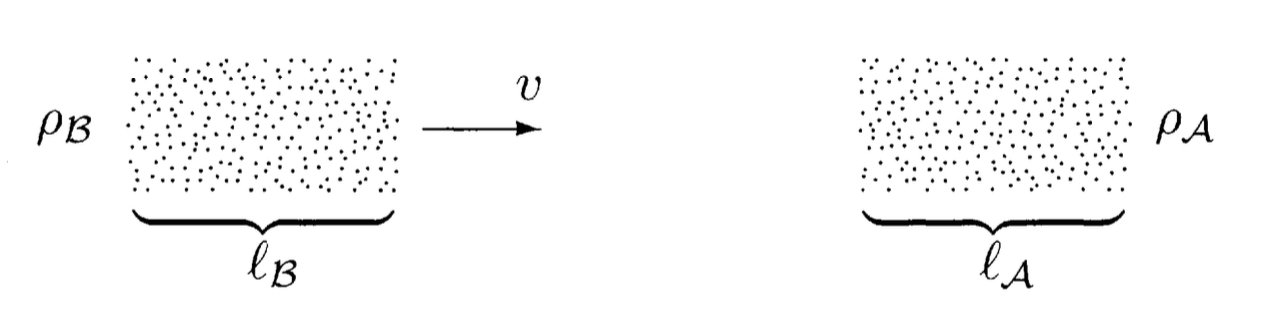
\includegraphics[width=0.8\textwidth]{figures/v.png}
\end{figure}


ここで $\ell_A$ と $\ell_B$ はそれぞれの粒子の束の長さとする。
すると散乱事象の全数(あるいは特定の型の散乱事象数)は
$\rho_A, \rho_B, \ell_A, \ell_B$ および二つの束に共通な断面積 $A$ に比例することが期待される。

したがって \textbf{断面積}($\sigma$ と書く)は、これらすべての量で割った散乱事象の全数として定義される:

\begin{equation}
\sigma \equiv
\frac{\text{Number of scattering events}}
{\rho_A \, \ell_A \, \rho_B \, \ell_B \, A}.
\tag{4.59}
\end{equation}

ここで, $N_A, N_B$ をそれぞれ粒子 $A, B$ の全数とする。  
散乱実験においては、様々な過程に対する断面積が関係してくる。  
例えば $e^+e^-$ 衝突では、$\mu^+\mu^-, \tau^+\tau^-, \mu^+\mu^-\gamma, \mu^+\mu^-\gamma\gamma$ など、ハドロン生成を含む無数の過程、さらには単純な $e^+e^-$ 散乱の断面積を測定できる。  
通常は、最終状態の粒子の種類だけでなく、それらがどの運動量で出てくるかも測定したい。

---

この場合、式 (4.59) の定義は依然として有効だが、運動量を正確に指定すると断面積 $\sigma$ は無限小になる。  
解決策は \textbf{微分断面積 (differential cross section)} を導入することである:

\[
\frac{d\sigma}{d^3p_1 \cdots d^3p_n}.
\]

これは、最終状態の運動量空間の領域に散乱する断面積を与える。  
最終状態の運動量は全て独立ではなく、4運動量保存則により4つの成分は常に拘束される。  
最も単純な場合、最終状態が2粒子しかない場合には、残る自由な成分は2つであり、通常は粒子の角度 $\theta,\phi$ ととられる。  
この場合、4つの拘束された成分に関して積分を行えば、通常の角度微分断面積 $d\sigma/d\Omega$ が得られる。

---

やや単純な測定可能量は \textbf{崩壊率 (decay rate)} $\Gamma$ である。  
これは静止している不安定粒子 $A$ が、特定の最終状態(2つ以上の粒子からなる)に崩壊する確率を表す。次のように定義される:

\begin{equation}
\Gamma \equiv 
\frac{\text{単位時間あたりの崩壊数}}
{\text{存在する $A$ 粒子の数}}.
\tag{4.62}
\end{equation}

粒子の寿命 $\tau$ は、全ての最終状態に対する崩壊率の総和の逆数である
(半減期は $\tau \cdot \ln 2$ である)。

---

非相対論的量子力学においては、不安定な原子状態は \textbf{共鳴 (resonance)} として散乱実験に現れる。  
共鳴エネルギー $E_0$ の近くでの散乱振幅は、Breit–Wigner 公式で与えられる:

\begin{equation}
f(E) \propto \frac{1}{E - E_0 + i\Gamma/2}.
\tag{4.63}
\end{equation}

したがって断面積は

\begin{equation}
\sigma \propto \frac{1}{(E - E_0)^2 + \Gamma^2/4}.
\end{equation}

となり、共鳴ピークの幅は不安定状態の崩壊率に等しい。

---

Breit–Wigner 公式 (4.63) は相対論的量子力学にも適用できる。  
特に、初期粒子が結合して不安定粒子を生成し、それが崩壊する過程の散乱振幅を与える。  
不安定粒子は真空の励起状態と見なすことができ、これは非相対論的な不安定原子状態の直接の類推である。  

不安定粒子 $p$ の4運動量を $p$、質量を $m$ とすると、(4.63) の相対論的不変化された一般化は次のようになる:

\begin{equation}
\frac{1}{p^2 - m^2 + im\Gamma}
\;\approx\;
\frac{1}{2E_p(p^0 - E_p + i(m/E_p)\Gamma/2)}.
\tag{4.64}
\end{equation}

一般の系における不安定粒子の崩壊率は、相対論的時間膨張に従って
\[
\frac{m}{E_p}\Gamma
\]
となる。  
式 (4.64) の二つの表現は共鳴付近では等しいが、左辺はローレンツ不変であり、はるかに便利である。

\section*{S行列}

では、どのようにして断面積を計算するのだろうか?  
我々はまず、初期状態の粒子を表す波束を設定し、この初期状態を相互作用場の時間発展演算子 $\exp(-iHt)$ により非常に長時間発展させ、その結果として得られる最終状態を、所望の最終状態粒子を表す波束と重ね合わせる必要がある。  
これにより、所望の最終状態が生成される確率振幅が得られ、断面積と直接関係する。  
波束が運動量空間で非常に狭い極限では、振幅は波束の形状ではなく、その運動量のみに依存することが分かる。  

---

ある状態 $|\phi\rangle$ を表す波束は次のように書ける:

\begin{equation}
|\phi\rangle = \int \frac{d^3k}{(2\pi)^3} \, \frac{1}{\sqrt{2E_{\mathbf{k}}}} \, \phi(\mathbf{k}) \, |\mathbf{k}\rangle,
\tag{4.65}
\end{equation}

ここで $\phi(\mathbf{k})$ は空間波動関数のフーリエ変換であり、$|\mathbf{k}\rangle$ は相互作用論における運動量 $\mathbf{k}$ の一粒子状態である。  
自由理論では $|\mathbf{k}\rangle = \sqrt{2E_{\mathbf{k}}}\, a^\dagger_{\mathbf{k}}|0\rangle$ である。  
因子 $\sqrt{2E_{\mathbf{k}}}$ によって相対論的規格化が通常の規格化に変換され、全ての確率の和が1になる:

\begin{equation}
\langle \phi | \phi \rangle = 1
\quad \text{ただし} \quad
\int \frac{d^3k}{(2\pi)^3} |\phi(\mathbf{k})|^2 = 1.
\tag{4.66}
\end{equation}

---

我々が計算したい確率は次である:

\begin{equation}
\mathcal{P} = \Big|\langle \underbrace{\phi_1 \phi_2 \cdots}_{\text{future}} 
\big| \underbrace{\phi_A \phi_B}_{\text{past}} \rangle \Big|^2,
\tag{4.67}
\end{equation}

ここで $|\phi_A \phi_B\rangle$ は過去の無限に遠い過去に構築された二つの波束状態であり、  
$\langle \phi_1 \phi_2 \cdots |$ は未来の無限に遠い未来に構築された複数の波束状態(各最終状態粒子ごとに一つ)である。  

波束は空間的に局在しているので、それぞれ独立して構築できる。  
このように構築された状態は \textbf{in状態} と \textbf{out状態} と呼ばれる。  
我々はハイゼンベルク描像を用いるので、状態は時間に依存しないが、状態に与える名前は時間依存演算子の固有値や期待値に依存する。  
したがって、異なる時刻で構築された状態は、演算子の時間依存性によって自明でない重なりを持つ。  

\begin{figure}[H]
    \centering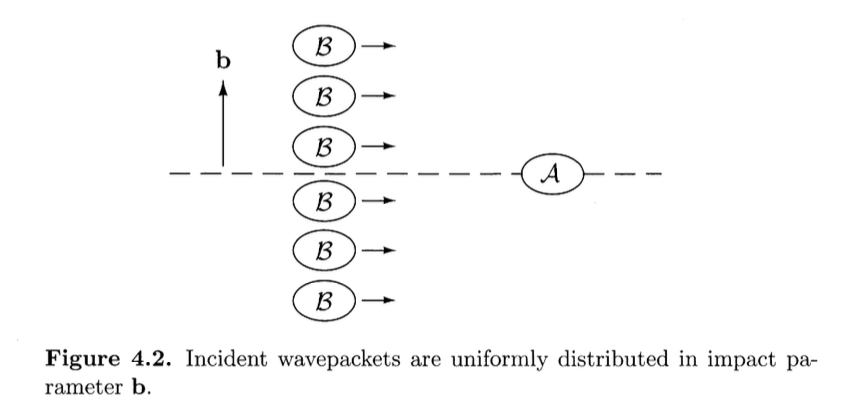
\includegraphics[width=0.8\textwidth]{figures/fig4.2.png}
\end{figure}

もし $|\phi_A \phi_B\rangle$ を過去の無限に遠い過去に設定し、波束 $\phi_i(\mathbf{k}_i)$ が特定の運動量 $\mathbf{p}_i$ のまわりに集中する極限をとれば、この状態は明確な初期運動量をもつ状態 $| \mathbf{p}_A \mathbf{p}_B\rangle_{\text{in}}$ を定義する。  
状態 $|\phi_A \phi_B\rangle$ をこのような状態の線形重ね合わせとして表すことは有用である. ただし, 位置空間における波束 $\phi_B$ が $\phi_A$ に対して横方向にずれていることを考慮することが重要である (図4.2参照).
位置空間でこの効果を考慮すると、$\phi_B(\mathbf{k}_B)$ に因子 $\exp(-i\mathbf{b}\cdot \mathbf{k}_B)$ を掛けて並進を表す。  
したがって、初期状態は次のように書ける:

\begin{equation}
|\phi_A \phi_B\rangle_{\text{in}}
= \int \frac{d^3k_A}{(2\pi)^3} \int \frac{d^3k_B}{(2\pi)^3} 
\frac{\phi_A(\mathbf{k}_A)\phi_B(\mathbf{k}_B)e^{-i\mathbf{b}\cdot \mathbf{k}_B}}
{\sqrt{(2E_A)(2E_B)}} \, |\mathbf{k}_A \mathbf{k}_B\rangle_{\text{in}} .
\tag{4.68}
\end{equation}

最終状態 $\langle \phi_1\phi_2\cdots|$ も同様に定義できる。  

\begin{equation}
\langle \phi_1\phi_2\cdots|_{\text{out}}
= \left( \prod_f \int \frac{d^3p_f}{(2\pi)^3}\frac{\phi_f(\mathbf{p}_f)}{\sqrt{2E_f}} \right) |\mathbf{p}_1 \mathbf{p}_2 \cdots \rangle_{\text{out}} .
\tag{4.69}
\end{equation}


散乱確率を実験的に測定可能な量として表すには、最終状態を運動量固有状態の \textbf{out状態} にとるのが便利である。  
その場合、(4.67) の確率は規格化因子を掛けて振幅の2乗を取ることで計算できる。  
これは、検出器が最終状態の粒子の運動量を測定するため、ドブロイ波長レベルでの位置分解能をもたないことを反映している。

従って散乱確率は、非現実的な波束状態ではなく、漸近的に定義された入出力状態の間の遷移確率として表される:

\begin{equation}
\langle \text{out} : \mathbf{p}_1 \mathbf{p}_2 \cdots | \mathbf{k}_A \mathbf{k}_B \rangle_{\text{in}}.
\tag{4.69}
\end{equation}


入出力状態の重ね合わせは、時間発展の極限で次のように定義される:

\begin{equation}
\langle \text{out} : \mathbf{p}_1 \mathbf{p}_2 \cdots | \mathbf{k}_A \mathbf{k}_B \rangle_{\text{in}}
= \lim_{T\to\infty} \langle \mathbf{p}_1 \mathbf{p}_2 \cdots | e^{-iH(2T)} | \mathbf{k}_A \mathbf{k}_B \rangle.
\tag{4.70}
\end{equation}

この極限で定義されるユニタリ演算子を \textbf{S行列} と呼ぶ:

\begin{equation}
\langle \text{out} : \mathbf{p}_1 \mathbf{p}_2 \cdots | \mathbf{k}_A \mathbf{k}_B \rangle_{\text{in}}
= \langle \mathbf{p}_1 \mathbf{p}_2 \cdots | S | \mathbf{k}_A \mathbf{k}_B \rangle.
\tag{4.71}
\end{equation}

---

$S$ 行列は次のような構造を持つ:相互作用が全くなければ $S=1$ であり、単なる恒等演算子である。  
相互作用がある場合には、粒子は単純に一方をすり抜けるだけでなく散乱する。  
このとき相互作用による寄与を抽出するために

\begin{equation}
S = 1 + iT
\tag{4.72}
\end{equation}

と定義する。

さらに $S$ の行列要素には4運動量保存の因子が必ず含まれるべきである。  
そこで \textbf{不変行列要素} $\mathcal{M}$ を次のように定義する:

\begin{equation}
\langle \mathbf{p}_1 \mathbf{p}_2 \cdots | iT | \mathbf{k}_A \mathbf{k}_B \rangle
= (2\pi)^4 \delta^{(4)}(k_A + k_B - \sum p_f) \; i\mathcal{M}(k_A, k_B \to p_f).
\tag{4.73}
\end{equation}

この $\mathcal{M}$ は非相対論的量子力学における散乱振幅に対応する。  
その有用性は、相互作用ハミルトニアンの詳細(dynamics)を含む物理を分離してくれる点にある。  


最後に、確率を具体的に計算しよう。  
初期状態 $|\phi_A \phi_B\rangle$ が、体積要素 $d^3p_1 \cdots d^3p_n$ に運動量を持つ $n$ 個の粒子を含む最終状態に散乱する確率は次である:

\begin{equation}
\mathcal{P}(AB \to 1 2 \cdots n) 
= \left( \prod_f \frac{d^3p_f}{(2\pi)^3 2E_f} \right)
\; \big| \langle \text{out} : \mathbf{p}_1 \cdots | \phi_A \phi_B \rangle_{\text{in}} \big|^2.
\tag{4.74}
\end{equation}

単一の標的粒子 $A$ と、多数の入射粒子 $B$ が異なるインパクトパラメータ $b$ をもって衝突する場合、  
散乱事象の数 $N$ は次のように書ける:

\begin{equation}
N = \sum_{\text{全入射粒子 } i} \mathcal{P}_i 
= \int d^2 b \, n_B \, \mathcal{P}(b),
\end{equation}

ここで $n_B$ は $B$ 粒子の数密度(単位面積あたりの数)である。  
相互作用範囲にわたって $n_B$ が一定であると仮定すると、これを積分の外に出せる。  
したがって断面積は

\begin{equation}
\sigma = \frac{N}{n_B N_A} = \frac{N}{n_B \cdot 1}
= \int d^2 b \, \mathcal{P}(b).
\tag{4.75}
\end{equation}

---

$\mathcal{M}$ を用いて $\sigma$ の表式を導出するのは比較的簡単である。  
(4.75), (4.74), (4.68) を組み合わせ($d\sigma$ と書く代わりに微小量と考える)、次を得る:

\begin{align}
d\sigma &= 
\left( \prod_f \frac{d^3p_f}{(2\pi)^3 \, 2E_f}\right)
\int d^2b \,
\left( \prod_{i=A,B} \frac{d^3k_i}{(2\pi)^3 \, \sqrt{2E_i}} \, \frac{d^3k'_i}{(2\pi)^3 \, \sqrt{2E'_i}} \right) \nonumber \\
&\qquad \times e^{i\mathbf{b}\cdot(\mathbf{k}_B - \mathbf{k}'_B)} 
\langle \text{out}(\{p_f\}) | \{k_i\}_{\text{in}} \rangle
\langle \{k'_i\}_{\text{in}} | \text{out}(\{p_f\}) \rangle.
\tag{4.76}
\end{align}

ここで $k_A, k_B$ をdummy変数として、振幅の絶対値の二乗に現れる。  
$b$ に関する積分を行うと、$\delta^{(2)}(\mathbf{k}_B - \mathbf{k}'_B)$ が生じる。  
また、最後の二つの因子を $\mathcal{M}$ で表すと:

\[
\langle \text{out}(\{p_f\}) | \{k_i\}_{\text{in}} \rangle 
= i\mathcal{M}(\{k_i\}\to\{p_f\})(2\pi)^4\delta^{(4)}\!\left(\sum k_i - \sum p_f\right),
\]

\[
\langle \{k'_i\}_{\text{in}} | \text{out}(\{p_f\}) \rangle 
= -i\mathcal{M}^*(\{k_i\}\to\{p_f\})(2\pi)^4\delta^{(4)}\!\left(\sum k'_i - \sum p_f\right).
\]

---

これら二つのデルタ関数を掛け合わせ、さらに $\delta^{(2)}(\mathbf{k}_B - \mathbf{k}'_B)$ を用いることで、  
6つの積分のうち4つは容易に実行できる。  
残りの2つの積分は次のように整理される:

\begin{align}
\int d\tilde{k}_A \, d\tilde{k}_B \, \delta^{(4)}(k_A+k_B-\sum p_f)
&= \int \frac{dE_A \, dE_B}{|\mathbf{v}_A - \mathbf{v}_B|} \, 
\delta(E_A+E_B-\sum E_f), \nonumber \\
&= \frac{1}{|\mathbf{v}_A - \mathbf{v}_B|},
\tag{4.77}
\end{align}

ここで $\mathbf{v}_A, \mathbf{v}_B$ はそれぞれの速度である。

---

以上をまとめると、断面積は次のように書ける:

\begin{align*}
d\sigma &=
\left( \prod_f \frac{d^3p_f}{(2\pi)^3 \, 2E_f} \right)
\frac{|\mathcal{M}(p_A,p_B\to\{p_f\})|^2}{2E_A 2E_B |\mathbf{v}_A - \mathbf{v}_B|}
\int \frac{d^3k_A}{(2\pi)^3} \frac{d^3k_B}{(2\pi)^3}\\
&\quad \times |\phi_A(\mathbf{k}_A)|^2 |\phi_B(\mathbf{k}_B)|^2 
(2\pi)^4 \delta^{(4)}(k_A+k_B-\sum p_f).
\tag{4.78}
\end{align*}

ここで初期波束が $p_A, p_B$ に集中していると仮定すると、上式は次のように簡単になる:

\begin{equation}
d\sigma =
\frac{1}{2E_A 2E_B |\mathbf{v}_A - \mathbf{v}_B|}
\left( \prod_f \frac{d^3p_f}{(2\pi)^3 \, 2E_f} \right)
|\mathcal{M}(p_A,p_B\to\{p_f\})|^2 
(2\pi)^4 \delta^{(4)}(p_A+p_B-\sum p_f).
\tag{4.79}
\end{equation}

---

最終状態の積分 measure は

\begin{equation}
d\Pi_n = 
\left( \prod_f \frac{d^3p_f}{(2\pi)^3 \, 2E_f} \right)
(2\pi)^4 \delta^{(4)}(P-\sum p_f),
\tag{4.80}
\end{equation}

で与えられる。ここで $P$ は初期4運動量である。  
この measure はローレンツ不変であり、$n$ 体位相空間 (invariant $n$-body phase space) と呼ばれる。  
したがって式 (4.79) のローレンツ変換特性は、前因子

\[
\frac{1}{E_A E_B |\mathbf{v}_A - \mathbf{v}_B|}
= \frac{1}{|E_{pA}\mathbf{p}_B - E_{pB}\mathbf{p}_A|}
= \frac{1}{\sqrt{(p_A\cdot p_B)^2 - m_A^2 m_B^2}}
\]

によって完全に決まる。  
これはローレンツ不変ではないが、$z$ 軸方向のboostに対しては不変である。  
実際には、この式は断面積の変換特性を表現する。

最終状態に2粒子しかない特別な場合、一般式 (4.79) を単純化できる。  
この場合、位相空間積分を重心系(center-of-mass frame)で評価する。  
2つの最終粒子を $p_1, p_2$ とし、三運動量保存のデルタ関数により $\mathbf{p}_2 = -\mathbf{p}_1$ が課される。  
すると二体位相空間要素は次の形になる:

\begin{equation}
d\Pi_2 = \frac{d^3p_1}{(2\pi)^3 2E_1} \frac{d^3p_2}{(2\pi)^3 2E_2}
(2\pi)^4 \delta(E_{\text{cm}} - E_1 - E_2),
\tag{4.81}
\end{equation}

ここで $E_1 = \sqrt{p_1^2 + m_1^2}, \, E_2 = \sqrt{p_2^2 + m_2^2}, \, E_{\text{cm}}$ は初期全エネルギーである。  

エネルギー保存のデルタ関数を積分すると:

\begin{equation}
d\Pi_2 = d\Omega \, \frac{|\mathbf{p}_1|^2}{16\pi^2 E_1 E_2} 
\left( \frac{p_1}{E_1} + \frac{p_1}{E_2} \right)^{-1}
= d\Omega \, \frac{|\mathbf{p}_1|}{16\pi^2 E_{\text{cm}}},
\tag{4.82}
\end{equation}

となる。ここで $d\Omega$ は立体角要素である。  

反応が衝突軸に対して対称な場合、二体位相空間は単純に極角積分で表せる:

\begin{equation}
d\Pi_2 = \frac{d\cos\theta}{16\pi} \frac{2|\mathbf{p}_1|}{E_{\text{cm}}}.
\tag{4.83}
\end{equation}

高エネルギーでは、この最後の因子は $1$ に近づく。  

---

この単純化を (4.79) に適用すると、二体散乱の断面積は次の形になる:

\begin{equation}
\left(\frac{d\sigma}{d\Omega}\right)_{\text{CM}}
= \frac{1}{2E_A 2E_B |\mathbf{v}_A - \mathbf{v}_B|}
\frac{|\mathbf{p}_1|}{(2\pi)^2 4E_{\text{cm}}}
|\mathcal{M}(p_A,p_B \to p_1,p_2)|^2.
\tag{4.84}
\end{equation}

---

特に全ての粒子が同じ質量(しばしば $m \to 0$ の極限を含む)ならば、この式は第1章で引用した結果に簡約される:

\begin{equation}
\left(\frac{d\sigma}{d\Omega}\right)_{\text{CM}}
= \frac{|\mathcal{M}|^2}{64\pi^2 E_{\text{cm}}^2}.
\tag{4.85}
\end{equation}

---

最後に、微分崩壊率 $d\Gamma$ の公式を導く。  
これは (4.79) の修正版として自然に導かれる。すなわち、$B$ 粒子が存在せず、単一粒子が崩壊する場合に対応する。  
このとき規格化因子 $(2E_A)^{-1}$ は $(2m_A)^{-1}$ に置き換わる(他の系では時間膨張を考慮する)。  
したがって崩壊率の公式は:

\begin{equation}
d\Gamma = \frac{1}{2m_A} \left( \prod_f \frac{d^3p_f}{(2\pi)^3 2E_f} \right)
|\mathcal{M}(m_A \to \{p_f\})|^2 (2\pi)^4 \delta^{(4)}(p_A - \sum p_f).
\tag{4.86}
\end{equation}

残念ながら、この公式の意味は必ずしも明確ではない。  
不安定粒子を無限に遠い過去へ送ることはできないため、我々の定義 (4.73) に基づいて  
$\mathcal{M}(m_A \to \{p_f\})$ を $S$ 行列で定義することは、この文脈では意味をなさない。  

それにもかかわらず、式 (4.86) は正しい。  
ただし $\mathcal{M}$ が、次節で述べる $S$ 行列要素に対するファインマンルールに従って計算された場合に限る。  
この点に関するさらなる議論、および式 (4.86) の厳密な証明は第7.3節まで延期する。  
それまでは、$\mathcal{M}$ を遷移振幅として直観的に理解することで十分である。  

---

式 (4.79) および (4.86) は完全に一般的であり、最終状態に複数の同一粒子が含まれるかどうかに依存しない。  
(もちろん $\mathcal{M}$ の計算は、同一粒子が存在する場合は異なるが、それはまた別の話である。)  

しかし、これらの公式を用いて断面積や崩壊率の \textbf{全体} を計算する際には、  
同じ最終状態を何度も数えてしまわないよう注意しなければならない。  

もし最終状態に $n$ 個の同一粒子が含まれるならば、積分を不等価な配置のみに制限するか、  
すべての運動量に対して積分した後に $n!$ で割る必要がある。







\end{document}
